

{

\addtobeamertemplate{background canvas}{\transfade[duration=0.001]}{}
%gets rid of bottom navigation bars
\setbeamertemplate{footline}[frame number]{}

%gets rid of bottom navigation symbols
\setbeamertemplate{navigation symbols}{}

%gets rid of footer
%will override 'frame number' instruction above
%comment out to revert to previous/default definitions
\setbeamertemplate{footline}{}

\begin{frame}{Fahrplanerstellungsproblem}
\textbf{Ziel}: Plane Kraftwerke so ein, dass sie die \alert{Last} gemeinsam erfüllen
\tikzset{
    trajectory/.style={issegrey},
    emph/.style={isseorange},
    trajectorynode/.style={issegrey},
    demand/.style={MidnightBlue, thick},
    firstTraj/.style={ForestGreen},
    secTraj/.style={BrickRed}
} 
\begin{figure}
\begin{tikzpicture}[scale=1.0]
    % Draw axes
    \draw [<->,thick] (0,5) node (yaxis) [above] {$P(t)$}
        |- (8.5,0) node (xaxis) [right] {$t$};
        
    \node[overlay,text width=1.9cm, text centered, anchor=south, right] at (7.7,4.5)
    { \small 
    \begin{itemize} 
    \item[] { \color{MidnightBlue} \onslide<2->{\textbf{Demand}} } 
    \item[] { \color{ForestGreen} \onslide<3->{Plant $a$} } 
    \item[] { \color{BrickRed} \onslide<4->{Plant $b$} }  
    \item[] { \color{isseorange} \onslide<5->{\textbf{Supply}} }    
    \end{itemize}
    };        
       
	
%	\node[text width = 1.5cm ,text centered, anchor=west, right] at (2.5, 1)
%	{
%		$\mathbf{+}$
%	};
	
    %\node[text width=2.5cm, text centered, anchor=west, right] at (4,-.5)
    %{
    %		Kraftwerk $\mathsf{b}$
	%}; 
	
	%\node[text width = 1.5cm ,text centered, anchor=west, right] at (6.5, 1)
	%{
	%	$\mathbf{=}$
%	};
	%\node[text width=2.5cm, text centered, anchor=west, right] at (8,-.5)
    %{
    %		Demand
	%};      
    
     % draw second trajectory first graph 
     \onslide<2->{
    \draw[trajectory,demand] (0,3.9) coordinate (d20) -- (1,4.6) coordinate (d21);
    \draw[trajectory,demand] (d21) -- (2,4.4) coordinate (d22);
    \draw[trajectory,demand] (d22) -- (3,4.7) coordinate (d23);
    \draw[trajectory,demand] (d23) -- (4,3.5) coordinate (d24);
    \draw[trajectory,demand] (d24) -- (5,3.5) coordinate (d25);
    \draw[trajectory,demand] (d25) -- (6,3.5) coordinate (d26);
    \draw[trajectory,demand] (d26) -- (7,4.0) coordinate (d27);
    \draw[trajectory,demand] (d27) -- (8,4.5) coordinate (d28);
    
    % now for the circles
    \fill[trajectorynode,demand] (d21) circle (1pt);
    \fill[trajectorynode,demand] (d22) circle (1pt);
    \fill[trajectorynode,demand] (d23) circle (1pt);
    \fill[trajectorynode,demand] (d24) circle (1pt);    
    \fill[trajectorynode,demand] (d25) circle (1pt);
    \fill[trajectorynode,demand] (d26) circle (1pt);
    \fill[trajectorynode,demand] (d27) circle (1pt);
    \fill[trajectorynode,demand] (d28) circle (1pt);
    }
        
    \onslide<3->{
    % now for the first plant   
    \draw[trajectory,firstTraj] (0,1.9) coordinate (p10) -- (1,2.0) coordinate (p11);
    \draw[trajectory,firstTraj] (p11) -- (2,2.4) coordinate (p12);
    \draw[trajectory,firstTraj] (p12) -- (3,2.4) coordinate (p13);
    \draw[trajectory,firstTraj] (p13) -- (4,2.2) coordinate (p14);
    \draw[trajectory,firstTraj] (p14) -- (5,2.4) coordinate (p15);
    \draw[trajectory,firstTraj] (p15) -- (6,2.4) coordinate (p16);
    \draw[trajectory,firstTraj] (p16) -- (7,2.4) coordinate (p17);                   
    \draw[trajectory,firstTraj] (p17) -- (8,2.6) coordinate (p18);
    
    	\onslide<6>{
       \draw[trajectory,firstTraj,very thick] (p11) -- (p12);	
       \node[overlay,align=left,rectangle callout,%
             callout absolute pointer=(p11.west),xshift=-.5cm,yshift=-1.5cm,fill=isseorange!50] at (p12) {
            \scriptsize \textbf{Must} ramp up \\ \scriptsize due to inertia};
       
	}    
    
 	\onslide<8>{
       \draw[trajectory,firstTraj,very thick] (p15) -- (p16);	
       \draw[trajectory,firstTraj,very thick] (p16) -- (p17);
       
          \node[overlay,align=left,rectangle callout,%
             callout absolute pointer=(p16.north),xshift=-.5cm,yshift=0.55cm,fill=isseorange!50] at (p15) {
           \scriptsize  Wait 2 steps for \\ \scriptsize further ramp-up};
	} 
	
    % now for the circles of the first graph
    \fill[trajectorynode,firstTraj] (p11) circle (1pt);
    \fill[trajectorynode,firstTraj] (p12) circle (1pt);
    \fill[trajectorynode,firstTraj] (p13) circle (1pt);
    \fill[trajectorynode,firstTraj] (p14) circle (1pt);    
    \fill[trajectorynode,firstTraj] (p15) circle (1pt);
    \fill[trajectorynode,firstTraj] (p16) circle (1pt);
    \fill[trajectorynode,firstTraj] (p17) circle (1pt);
    \fill[trajectorynode,firstTraj] (p18) circle (1pt);        
    }
    
    \onslide<4->{
    % now for the second plant   
    \draw[trajectory,secTraj] (0,2.0) coordinate (p20) -- (1,2.6) coordinate (p21);
    \draw[trajectory,secTraj] (p21) -- (2,2.0) coordinate (p22);
    \draw[trajectory,secTraj] (p22) -- (3,2.2) coordinate (p23);
    \draw[trajectory,secTraj] (p23) -- (4,1.5) coordinate (p24);
    \draw[trajectory,secTraj] (p24) -- (5,1.4) coordinate (p25);
    \draw[trajectory,secTraj] (p25) -- (6,1.2) coordinate (p26);
    \draw[trajectory,secTraj] (p26) -- (7,1.6) coordinate (p27);                   
    \draw[trajectory,secTraj] (p27) -- (8,1.9) coordinate (p28);
	\onslide<6>{
       \draw[trajectory,secTraj,very thick] (p21) -- (p22);	
       \node[overlay,align=left,rectangle callout,%
             callout absolute pointer=(p21.north),xshift=+1cm,yshift=.5cm,fill=isseorange!50] at (p21) {
            \scriptsize Has to compensate};
	}    
	
	\onslide<7>{
       \draw[trajectory,secTraj,very thick] (p23) -- (p24);	
       \node[overlay,align=left,rectangle callout,%
             callout absolute pointer=(p24.south),xshift=+1cm,yshift=-.8cm,fill=isseorange!50] at (p24) {
             \scriptsize Cannot ramp down further};
	}    
    
     % now for the circles of the second graph
    \fill[trajectorynode,secTraj] (p21) circle (1pt);
    \fill[trajectorynode,secTraj] (p22) circle (1pt);
    \fill[trajectorynode,secTraj] (p23) circle (1pt);
    \fill[trajectorynode,secTraj] (p24) circle (1pt);    
    \fill[trajectorynode,secTraj] (p25) circle (1pt);
    \fill[trajectorynode,secTraj] (p26) circle (1pt);
    \fill[trajectorynode,secTraj] (p27) circle (1pt);
    \fill[trajectorynode,secTraj] (p28) circle (1pt);
    }
    
    \onslide<5->{
    % draw joint production first graph 
    \draw[trajectory,emph] (0,3.9) coordinate (s20) -- (1,4.6) coordinate (s21);
    \draw[trajectory,emph] (s21) -- (2,4.4) coordinate (s22);
    \draw[trajectory,emph] (s22) -- (3,4.6) coordinate (s23);
    \draw[trajectory,emph] (s23) -- (4,3.7) coordinate (s24);
    \draw[trajectory,emph] (s24) -- (5,3.8) coordinate (s25);
    \draw[trajectory,emph] (s25) -- (6,3.6) coordinate (s26);
    \draw[trajectory,emph] (s26) -- (7,4.0) coordinate (s27);
    \draw[trajectory,emph] (s27) -- (8,4.5) coordinate (s28);
    
	% now for the circles of the sum
    \fill[trajectorynode,emph] (s21) circle (1pt);
    \fill[trajectorynode,emph] (s22) circle (1pt);
    \fill[trajectorynode,emph] (s23) circle (1pt);
    \fill[trajectorynode,emph] (s24) circle (1pt);    
    \fill[trajectorynode,emph] (s25) circle (1pt);
    \fill[trajectorynode,emph] (s26) circle (1pt);
    \fill[trajectorynode,emph] (s27) circle (1pt);
    \fill[trajectorynode,emph] (s28) circle (1pt);
    }
    
	\node[text centered, anchor=north] at (1,0) { 1 }; \draw[thick] (1,0.05) -- (1,-.05);
	\node[text centered, anchor=north] at (2,0) { 2 }; \draw[thick] (2,0.05) -- (2,-.05);
	\node[text centered, anchor=north] at (3,0) { 3 }; \draw[thick] (3,0.05) -- (3,-.05);	
	\node[text centered, anchor=north] at (4,0) { 4 }; \draw[thick] (4,0.05) -- (4,-.05);
	\node[text centered, anchor=north] at (5,0) { 5 }; \draw[thick] (5,0.05) -- (5,-.05);
	\node[text centered, anchor=north] at (6,0) { 6 }; \draw[thick] (6,0.05) -- (6,-.05);
	\node[text centered, anchor=north] at (7,0) { 7 }; \draw[thick] (7,0.05) -- (7,-.05);	
	\node[text centered, anchor=north] at (8,0) { 8 }; \draw[thick] (8,0.05) -- (8,-.05);
	    

\end{tikzpicture}
\end{figure}  
\end{frame}
}


\begin{frame}{Hierarchisches Energiemanagement} \large

\begin{figure}
\centering
\begin{tikzpicture}[->,>=stealth',shorten >=1pt,auto,node distance=1.3cm,
  thick,main node/.style={circle,fill=black!15,draw,font=\sffamily}]

 \node[hierNode, double, label=north:\only<1->{500}] (tl) {a};
 \node[hierNode, double,label=west:\only<4->{\alert<4>{300}}] (i) [xshift=-.2cm, yshift=-.3cm,below left of=tl] {\alert<3-4>{i}}; 
 \node[hierNode, double,label=east:\only<4->{\alert<4>{200}}] (j) [below right of=tl,yshift=-.3cm,xshift=.9cm] {\alert<3-4>{j}};


 \node[hierNode, cStyle, label=south:\only<8->{60}] (c) [below of=i] {\alert<5-7>{c}}; 
 
 \node[hierNode,bStyle, label=south:\only<8->{140}] (b) [left of=c] {\alert<5-7>{b}}; 
 \node[hierNode, dStyle, label=south:\only<8->{100}] (d) [right of=c] {\alert<5-7>{d}}; 
 \node[hierNode, bStyle, label=south:\only<8->{160}] (e) [right of=d] {\alert<5-7>{e}}; 
 \node[hierNode, dStyle, label=south:\only<8->{40}] (f) [right of=e] {\alert<5-7>{f}}; 
  
 
  \path[every node/.style={font=\sffamily\tiny}]
    (tl) edge node [right] {} (i)
   	     edge node [right] {} (j) 
   	(i) edge node [right] {} (b)
   	     edge node [right] {} (c)
   	     edge node [right] {} (d) 
   	(j) edge node [right] {} (e)
   	     edge node [right] {} (f)      ;   	     
  
\onslide<2-4>{ \node[optboundaries, text width=13.5em, text height = 6.4em] (tlOpt) at (.4,-.4) { };}  
 
\onslide<5->{\node[optboundaries, text width=8.7em, text height = 6.8em] (iOpt) at (-1.2,-2.0) {}; }
 
\onslide<5->{\node[optboundaries, text width=6.3em, text height = 6.8em] (jOpt) at (2.2,-2.0) {};}  
 

\onslide<3-4,9->{  
\node[overlay,align=left,rectangle callout,%
      callout absolute pointer=(tl.west),fill=isseorange!50] at (-3.8,-0.3) {Was sollen $i$ und $j$\\ beisteuern?};} 
     
\onslide<4,9->{     
\node[overlay,rectangle callout,%
      callout absolute pointer=(j.north),fill=isseorange!50] at (3.0,1.4) {Wie kann ich $e$ und $f$ repräsentieren?}; } 

\onslide<6->{
\node[overlay,align=left,rectangle callout,%
      callout absolute pointer=(b.west),fill=isseorange!50] at (-3.8,-4.3) {Wie vermeide ich \\ meinen Speicher \\über 90\% zu füllen?}; } 
      
\onslide<7-> { \node[overlay,align=left,rectangle callout,%
      callout absolute pointer=(f.east),fill=isseorange!50] at (4.3,-4.4) {Wie beschreibe ich \\meine Abläufe?}; }
      
\onslide<10-> { \node[overlay,align=left, fill=issegrey!20] at (0.3,-4.4) {\footnotesize Constraint Relationships / PVS \\
\footnotesize \CustomCite{SGAI'13}, \CustomCite{ICTAI'14} \\
\footnotesize \CustomCite{Wirsing'15}, \alert{\CustomCite{Constraints'16}}
}; }      

\onslide<11-> { \node[overlay,align=left, fill=issegrey!20] at (-3.2,1.4) {\footnotesize Regio-zentrale Fahrpläne\\
\footnotesize \CustomCite{ICAART'14}, \CustomCite{SAOS'14} \\
\footnotesize Marktbasiert \\
\footnotesize \CustomCite{TAAS'15}
}; }      

\onslide<12-> { \node[overlay,align=left, fill=issegrey!20] at (4.7,0.2) {\footnotesize Abstraktion\\
\footnotesize \CustomCite{ICAART'14}, \CustomCite{TCCI'15} \\
\footnotesize \CustomCite{SASO'15}
}; }  

\onslide<13-> { \node[overlay,align=left, fill=issegrey!20] at (5.3,-2.0) {\footnotesize Supply Automata \\
\footnotesize \CustomCite{SEN-MAS'14} \\
\footnotesize \CustomCite{TCCI'15}
}; }  
\end{tikzpicture}

\label{fig:hierarchical-decomposition}
\end{figure}
\end{frame}


\begin{frame}{Soft Constraints} \large
\begin{figure}
\centering
  
\pgfdeclarelayer{background}
\pgfdeclarelayer{foreground}
\pgfsetlayers{background,main,foreground}
\begin{tikzpicture}[->,>=stealth',shorten >=1pt,auto,node distance=1.3cm,
  thick,main node/.style={circle,fill=black!15,draw,font=\sffamily}]

\node[hierNode, double,label=east:300] (i) [xshift=-.2cm, yshift=-.3cm] {i}; 
\node[hierNode, cStyle, label=south:60] (c) [below of=i] {c}; 
\node[hierNode,bStyle, label=south:140] (b) [left of=c] {b}; 
\node[hierNode, dStyle, label=south:100] (d) [right of=c] {d}; 

 
  \path[every node/.style={font=\sffamily\tiny}]
   (i) edge node [right] {} (b)
   	     edge node [right] {} (c)
   	     edge node [right] {} (d)      ;   	     
  
 
\node[optboundaries, text width=8.9em, text height = 6.8em] (jOpt) at (-0.2,-1.0) {};  
 
      
\node[overlay,align=left,rectangle callout,%
      callout absolute pointer=(b.north),fill=isseorange!50] (bubble) at (-0.4,1.4) {Wie vermeide ich \\ meinen Speicher \\über 90\% zu füllen?}; 

\onslide<2->{      
\node[align=left,rectangle,dashed,rounded corners, rectangle callout, text width = 6cm, text height = 5.5cm,
      callout absolute pointer=(bubble.east),fill=black!5] at (6.5,-1.4) {}; 
};

\pgfmathsetmacro{\XOr}{5.3}
\pgfmathsetmacro{\YOr}{-1.2}
\pgfmathsetmacro{\YHeight}{2}
\pgfmathsetmacro{\XWidth}{2.5}
\pgfmathsetmacro{\YXOr}{(\YOr + \YHeight}
\pgfmathsetmacro{\XYOr}{(\XOr + \XWidth}

\coordinate (origin) at (\XOr,\YOr);
\coordinate (originX) at (\XOr,\YXOr);
\coordinate (originY) at (\XYOr,\YOr);

\onslide<3->{      

}


 \begin{pgfonlayer}{foreground}
 \tikzset{
   main node/.style={rectangle,
                     rounded corners,
   					 fill=black!15,
   					 draw,
   					 minimum width=3.5em,
   					 text centered,
                     inner sep=2.5pt,	 
   					 font=\sffamily
   					},
   treestyle/.style={rectangle,fill=black!15,draw,font=\sffamily},
   constraint/.style={circle,fill=black!15,draw,font=\sffamily\small},
   constraint_satisfied/.style = {constraint, fill=white},
   constraint_violated/.style = {constraint, fill=black!25},
}

       \tikzstyle{every state}=[circle,fill=black!25,minimum size=17pt,inner sep=.2pt]
\onslide<3->{      
\draw [black!85,fill=white] (5.0,0.5) rectangle (9.0,-1.8);
\node[main node, style={font=\sffamily\footnotesize}] (5) at (7.05,-0.2) {\gasFull};
\node[main node, style={font=\sffamily\footnotesize}] (6) [below left of=5,xshift=-1.4] {\ecoSweet};
\node[main node, style={font=\sffamily\footnotesize}] (7) [below right of=5,xshift=2.1] {\onOff};
%\node[main node, style={font=\sffamily\footnotesize},double] (hardConstraint) [below left of=7,xshift=-3.1,yshift=7] {$\mathsf{maxProd}$};

%\node[text width=2cm, anchor=west, left] at (7.2, -1.8) { \textsc{TPD} };

\path[every node/.style={font=\sffamily\tiny}]
  (6) edge node [right] {} (5)
  (7) edge node [right] {} (5)
;
}
%
%\node[overlay] at (6.5, 0.0) {
%\only<4->{      
% 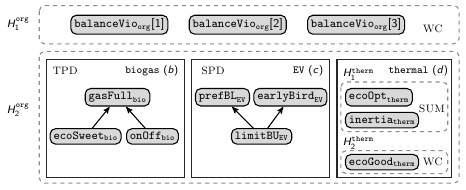
\includegraphics[width=.4\textwidth]{img/pvs.png} } };
% 
    \end{pgfonlayer}

\end{tikzpicture}

\end{figure}
\vspace*{-2.4ex}
\onslide<5->{\textbf{Ziel:} Integration von Individualpräferenzen.}
\end{frame}

\begin{frame}
\frametitle{Präferenzen im Constraint-Solving}

Constraint-Problem $((X, D), C)$
\begin{itemize}
  \item \cemph{Variablen} $X$,
\cemph{Domänen} $D = (D_x)_{x \in X}$,
\cemph{Constraints} $C$
\end{itemize}

\vspace*{1ex}

In der Praxis: \cemph{unerfüllbare} Probleme

\vspace*{2ex}

$((\{ \mathrm{x}, \mathrm{y}, \mathrm{z} \},
\mathrm{D}_{\mathrm{x}} = \mathrm{D}_{\mathrm{y}} =
\mathrm{D}_{\mathrm{z}} = \{ 1, 2, 3 \}), \{ \mathrm{c}_1,
\mathrm{c}_2, \mathrm{c}_3 \})$ mit
\bgroup\abovedisplayskip4pt\belowdisplayskip4pt
\begin{align*}
  \mathrm{c}_1 &: \mathrm{x} + 1 = \mathrm{y}
\\[-.4ex]
  \mathrm{c}_2 &: \mathrm{z} = \mathrm{y} + 2
\\[-.4ex]
  \mathrm{c}_3 &: \mathrm{x} + \mathrm{y} \leq 3
\end{align*}
\egroup

\begin{itemize}
  \item Nicht alle Constraints können gleichzeitig erfüllt werden
\begin{itemize}
  \item z.\,B., $\mathrm{c}_2$ erzwingt $\mathrm{z} = 3$ und $\mathrm{y} = 1$, im Konflikt zu $\mathrm{c}_1$
\end{itemize}

  \item Ein Agent wählt also zwischen Belegungen, die $\{ \mathrm{c}_1, \mathrm{c}_3 \}$ oder $\{ \mathrm{c}_2, \mathrm{c}_3 \}$ erfüllen.
\end{itemize}

\vspace*{2ex}

Welche Belegungen $v \in [X \to D]$ sollen \cemph{bevorzugt} werden?

\end{frame}


\begin{frame}{(Soft) Constraints in der Energie}

\alert{Harte} Constraints aus Supply Automata:
\begin{equation}
\mathsf{hardBounds}: \forall t \in T, a \in A : m[a][t] = \mathsf{on} \rightarrow P_{\mathrm{min}} \leq S[a][t] \leq P_{\mathrm{max}} \nonumber
\end{equation}

\pause
\vspace*{2ex}
\alert{Weiche} Constraints anlagenspezifisch (z.B. Präferenz für 350 bis 390 KW):
\begin{equation}
\mathsf{ecoSweet}_{\mathsf{bio}}: \forall t \in T : m[\mathsf{biogas}][t] = \mathsf{on} \rightarrow 350 \leq S[\mathsf{biogas}][t] \leq 390 \nonumber
\end{equation}

\pause
\vspace*{2ex}
oder Änderungsgeschwindigkeit
\begin{equation}
\mathsf{inertia}_{\mathsf{therm}}: \forall t \in T : |S[\mathsf{biogas}][t] - S[\mathsf{biogas}][t+1] | \leq 10 \nonumber
\end{equation}
\end{frame}

% block styles
\tikzstyle{sensor}=[draw, fill=blue!20, text width=5em, 
    text centered, minimum height=2.5em,drop shadow]    
    
\tikzstyle{alg} = [sensor, text width=5em, fill=isseorange!20, 
    minimum height=13em, rounded corners, drop shadow]
\tikzstyle{constraint}=[draw, circle, fill=issegrey!20, text width=1.2em, 
    text centered, minimum height=1.5em,drop shadow]
\tikzstyle{domainstore} = [alg, text width=5em, fill=isseorange!40, 
    minimum height=4em, rounded corners]
\tikzstyle{goodc} = [ForestGreen, font=\bfseries]
\tikzstyle{badc} = [Red, font=\bfseries]
\tikzstyle{okayc} = [LimeGreen, font=\bfseries]
        
\tikzset{
vecArrow/.style={
  thick
  }
}

\tikzset{
    mynode/.style={rectangle,rounded corners,draw=black, top color=isseorange!5, bottom color=isseorange!30,
                   very thick, inner sep=\myinnersep*1em, minimum size=3em, text centered, outer sep=0, align=center},
    innernode/.style={mynode, text width=3cm,  minimum height=1.5cm,
                      top color=issegrey!20, bottom color=issegrey!60},
    emphnode/.style={innernode, top color=isseorange!30, bottom color=isseorange!70}
}

% Define distances for bordering
\def\blockdist{2.3}
\def\edgedist{2.5}

  \tikzset{
    invisible/.style={opacity=0},
    visible on/.style={alt={#1{}{invisible}}},
    alt/.code args={<#1>#2#3}{%
      \alt<#1>{\pgfkeysalso{#2}}{\pgfkeysalso{#3}} % \pgfkeysalso doesn't change the path
    },
  }
%  
%\begin{frame}{Traditionelles Constraint-Solving}
%\fontsize{8pt}{7.2}\selectfont
%\begin{center}
%\begin{tikzpicture}
%% First row:
% \node (search) [alg]  {Suche \phantom{$x = 5$} };
% \path (search.east)+(4.6,0) node (propag) [alg,text width =12em]  {};
% \node[below right] at (propag.north west) {Constraint Store $C$};
% 
% \path (propag.west)+(0.8,-1.2) node (c1) [constraint] {$c_1$}; 
% \path (propag.west)+(1.1,-0.2) node (c2) [constraint] {$c_2$}; 
% \path (propag.west)+(2.0,0.4) node (c3) [constraint] {$c_3$}; 
% \path (propag.west)+(3.2,0.7) node (c4) [constraint] {$c_4$};
%  
% \path (propag.east)+(-1.2,-1.2) node (domainstore) [domainstore] {Domain Store $(D_x)_{x \in X}$}; 
% 
% \path [draw,vecArrow, ->] ([yshift=-2em]search.north east) -- node [above,visible on=<2->] {$x\gets5$} ([yshift=-2em]propag.north west);
% \path [draw,vecArrow, <-] ([yshift=2em]search.south east) -- node [above,goodc,visible on=<4->] {$\top$} ([yshift=2em]propag.south west);
% 
% \path [draw, vecArrow, <->] (c1.east) -- node [below,visible on=<3->,goodc] {$\top$} (domainstore.west) ;
% \path [draw,vecArrow, <->] (c2.330) -- node [above right,visible on=<3->,goodc] {$\top$} (domainstore.150) ;
% \path [draw,vecArrow, <->] (c3.290) -- node [right,visible on=<3->,goodc] {$\top$} (domainstore.120) ;
% \path [draw,vecArrow, <->] (c4.south) -- node [right,visible on=<3->,goodc] {$\top$} (domainstore.68) ;
%\end{tikzpicture}
%\end{center}
%\onslide<0>{
%\begin{columns}[c] % contents are top vertically aligned
%     \begin{column}[c]{7cm} % each column can also be its own 
%\begin{itemize}
%\item A set of satisfaction degrees $\mathbb{B} = \{ \bot, \top \}$
%\item A combination operation $\wedge$
%\item A neutral element $\top$
%\item A partial order $(\mathbb{B}, \leq_\mathbb{B})$ with $\top <_\mathbb{B} \bot$.
%\end{itemize}
%\end{column}
%     \begin{column}[c]{4.5cm} 
%     \end{column} 
%\end{columns}
%}
%
%\end{frame}
%
%\begin{frame}{Traditionelles Constraint-Solving}
%\fontsize{8pt}{7.2}\selectfont
%\begin{center}
%\begin{tikzpicture}
%% First row:
% \node (search) [alg]  {Suche $x = 5$};
% \path (search.east)+(4.6,0) node (propag) [alg,text width =12em]  {};
% \node[below right] at (propag.north west) {Constraint Store $C$};
% 
% \path (propag.west)+(0.8,-1.2) node (c1) [constraint] {$c_1$}; 
% \path (propag.west)+(1.1,-0.2) node (c2) [constraint] {$c_2$}; 
% \path (propag.west)+(2.0,0.4) node (c3) [constraint] {$c_3$}; 
% \path (propag.west)+(3.2,0.7) node (c4) [constraint] {$c_4$};
%  
% \path (propag.east)+(-1.2,-1.2) node (domainstore) [domainstore] {Domain Store $(D_x)_{x \in X}$}; 
% 
% \path [draw,vecArrow, ->] ([yshift=-2em]search.north east) -- node [above,visible on=<2->] {$y \gets 4$} ([yshift=-2em]propag.north west);
% \path [draw,vecArrow, <-] ([yshift=2em]search.south east) -- node [below,badc,visible on=<4->] {$\bot$} ([yshift=2em]propag.south west);
% 
% \path [draw, vecArrow, <->] (c1.east) -- node [below,visible on=<3->,badc] {$\bot$} (domainstore.west) ;
% \path [draw,vecArrow, <->] (c2.330) -- node [above right,visible on=<3->,goodc] {$\top$} (domainstore.150) ;
% \path [draw,vecArrow, <->] (c3.290) -- node [right,visible on=<3->,goodc] {$\top$} (domainstore.120) ;
% \path [draw,vecArrow, <->] (c4.south) -- node [right,visible on=<3->,goodc] {$\top$} (domainstore.68) ;
%\end{tikzpicture}
%\end{center}
%\onslide<5->{
%\begin{columns}[c] % contents are top vertically aligned
%     \begin{column}[c]{7cm} % each column can also be its own 
%\begin{itemize}
%
%\item Eine Menge von Bewertungen $\mathbb{B} = \{ \bot, \top \}$
%\item Eine Kombination $\wedge$
%\item Ein neutrales Element $\top$
%\item Eine partielle Ordnung $(\mathbb{B}, \leq_\mathbb{B})$ with $\top <_\mathbb{B} \bot$.
%\end{itemize}
%   \end{column} 
%     \begin{column}[c]{4.5cm} 
%     \end{column} 
%\end{columns}
%}
%\end{frame}

\begin{frame}{Soft-Constraint-Solving}
\fontsize{8pt}{7.2}\selectfont
\begin{center}
\begin{tikzpicture}
% First row:
 \node (search) [alg]  {Search $x = 5$};
 \path (search.east)+(4.6,0) node (propag) [alg,text width =12em]  {};
 \node[below right] at (propag.north west) {Constraint Store $C$};
 
 \path (propag.west)+(0.8,-1.2) node (c1) [constraint] {$c_1$}; 
 \path (propag.west)+(1.1,-0.2) node (c2) [constraint] {$c_2$}; 
 \path (propag.west)+(2.0,0.4) node (c3) [constraint] {$c_3$}; 
 \path (propag.west)+(3.2,0.7) node (c4) [constraint] {$c_4$};
  
 \path (propag.east)+(-1.2,-1.2) node (domainstore) [domainstore] {Domain Store $(D_x)_{x \in X}$}; 
 
 \path [draw,vecArrow, ->] ([yshift=-2em]search.north east) -- node [above,visible on=<2->] {$y \gets 4$} ([yshift=-2em]propag.north west);
 \path [draw,vecArrow, <-] ([yshift=2em]search.south east) -- node [below,okayc,visible on=<4->] {$4$} ([yshift=2em]propag.south west);
 
 \path [draw, vecArrow, <->] (c1.east) -- node [below,visible on=<3->,okayc] {$4$} (domainstore.west) ;
 \path [draw,vecArrow, <->] (c2.330) -- node [above right,visible on=<3->,goodc] {$0$} (domainstore.150) ;
 \path [draw,vecArrow, <->] (c3.290) -- node [right,visible on=<3->,goodc] {$0$} (domainstore.120) ;
 \path [draw,vecArrow, <->] (c4.south) -- node [right,visible on=<3->,goodc] {$0$} (domainstore.68) ;
\end{tikzpicture}
\end{center}
\onslide<5->{
\begin{columns}[c] % contents are top vertically aligned
     \begin{column}[c]{7cm} % each column can also be its own environment
    \begin{itemize}
\item Eine Menge von Bewertungen, z.B., $\{ 0, \ldots, k \}$
\item Eine Kombination $+$
\item Ein neutrales Element $0$
\item Eine partielle Ordnung $(\mathbb{N}, \geq)$ mit $0$ als Top 
\end{itemize}
   \end{column} \pause
     \begin{column}[c]{4.5cm} 
        Genannt \cemph{valuation structure}~\cite{Schiex1995valued}, bei totaler Ordnung, ansonsten \cemph{partial valuation structure}~\cite{Gadducci2013}.
        Ähnlich:  \cite{Bistarelli1999}: c-Semiringe 
     \end{column}
\end{columns}
    
}
\end{frame}


\begin{frame}{Partial Valuation Structures}
Zugrundeliegende \alert{algebraische Struktur}: Partielle Bewertungsstruktur (\emph{partial valuation structure, partiell geordnetes, kommutatives Monoid)}
\begin{itemize}
\item $(M, \cdot_M, \varepsilon_M, \leq_M)$ 
\item $m \cdot_m \varepsilon_M = m$
\item $m \leq_M \varepsilon_M$ ($\varepsilon_M = \top_M$)
\item $m \leq_M n \rightarrow m \cdot_M o \leq_M n \cdot_M o$
\end{itemize}
\vspace*{2ex}

\begin{columns}[onlytextwidth,T]
    
    \begin{column}{.7\textwidth}
          
    \hSecond{Abstrakt}
    
    \begin{itemize}
    \item $M$ \ldots Elemente
    \item $\cdot_M$ \ldots Kombination von Bewertungen
    \item $\varepsilon_M$ \ldots neutrales, ``bestes'' Element
    \item $\leq_M$ \ldots Ordnung, links ``schlechter''
    \end{itemize}
    \end{column}
    
    \begin{column}{.3\textwidth}
  	\hFirst{Konkret}  
  	 \begin{itemize}
    \item $\{0, \ldots, k \}$ 
    \item $+_k$
    \item $0$ 
    \item $\geq$
    \end{itemize}
    \end{column}
  \end{columns}

  \vspace*{2ex}
  
  \hfill \emph{\cite{Gadducci2013,SchiendorferPvs2015}}
\end{frame}


\begin{frame}[fragile]{PVS--Idee}
\begin{center}
\begin{tabular}{l|c|c|c|c}
\textbf{Konkrete PVS-Typen} & $M$ & $\cdot_M$ & $\leq_M$ & $\varepsilon_M$ \\ 
\hline 
Weighted CSP (WCSP)& $\mathbb{N}$ & $+$ & $\geq$ & $0$ \\ 
Cost Function Network (CFN)& $\{0,\ldots,k\}$ & $+$/$\max$ & $\geq$ & $0$ \\ 
Fuzzy CSP & $[0,1]$ & $\min$ & $\leq$  & 1 \\ 
Inclusion Max CSP & $2^{C_s}$ & $\cup$ & $\supseteq$  & $\emptyset$ \\ 
Constraint Relationships (CR)\footnote{$C_s$ is the set of soft constraints, $\supseteq_{\mathsf{SPD}}$ is the SPD-ordering on sets.} &$\mathcal{M}^{\mathrm{fin}} (C_s)$ & $\mcup$ & $\supseteq_{\mathsf{SPD}}$ & $\lbag \rbag$ \\ 
\end{tabular} 
\end{center}

\begin{parchment}[Hauptidee]
Implementiere Lösungsverfahren für Constraint-Probleme, die durch Bewertungsstrukturen geordnet sind. Instantiiere für konkrete Probleme.
\end{parchment}
\end{frame}

\begin{frame}{Soft Constraints} \large
\begin{figure}
\centering
  
\pgfdeclarelayer{background}
\pgfdeclarelayer{foreground}
\pgfsetlayers{background,main,foreground}
\begin{tikzpicture}[->,>=stealth',shorten >=1pt,auto,node distance=1.3cm,
  thick,main node/.style={circle,fill=black!15,draw,font=\sffamily}]

\node[hierNode, double,label=east:300] (i) [xshift=-.2cm, yshift=-.3cm] {i}; 
\node[hierNode, cStyle, label=south:60] (c) [below of=i] {c}; 
\node[hierNode,bStyle, label=south:140] (b) [left of=c] {b}; 
\node[hierNode, dStyle, label=south:100] (d) [right of=c] {d}; 

 
  \path[every node/.style={font=\sffamily\tiny}]
   (i) edge node [right] {} (b)
   	     edge node [right] {} (c)
   	     edge node [right] {} (d)      ;   	     
  
 
\node[optboundaries, text width=8.9em, text height = 6.8em] (jOpt) at (-0.2,-1.0) {};  
 
      
\node[overlay,align=left,rectangle callout,%
      callout absolute pointer=(b.north),fill=isseorange!50] (bubble) at (-0.4,1.4) {Wie vermeide ich \\ meinen Speicher \\über 90\% zu füllen?}; 

\onslide<2->{      
\node[align=left,rectangle,dashed,rounded corners, rectangle callout, text width = 6cm, text height = 5.5cm,
      callout absolute pointer=(bubble.east),fill=black!5] at (6.5,-1.4) {}; 
};

\pgfmathsetmacro{\XOr}{5.3}
\pgfmathsetmacro{\YOr}{-1.2}
\pgfmathsetmacro{\YHeight}{2}
\pgfmathsetmacro{\XWidth}{2.5}
\pgfmathsetmacro{\YXOr}{(\YOr + \YHeight}
\pgfmathsetmacro{\XYOr}{(\XOr + \XWidth}

\coordinate (origin) at (\XOr,\YOr);
\coordinate (originX) at (\XOr,\YXOr);
\coordinate (originY) at (\XYOr,\YOr);

\onslide<3->{      

}


 \begin{pgfonlayer}{foreground}
 \tikzset{
   main node/.style={rectangle,
                     rounded corners,
   					 fill=black!15,
   					 draw,
   					 minimum width=3.5em,
   					 text centered,
                     inner sep=2.5pt,	 
   					 font=\sffamily
   					},
   treestyle/.style={rectangle,fill=black!15,draw,font=\sffamily},
   constraint/.style={circle,fill=black!15,draw,font=\sffamily\small},
   constraint_satisfied/.style = {constraint, fill=white},
   constraint_violated/.style = {constraint, fill=black!25},
}

       \tikzstyle{every state}=[circle,fill=black!25,minimum size=17pt,inner sep=.2pt]
\onslide<3->{      
\draw [black!85,fill=white] (5.0,0.5) rectangle (9.0,-1.8);
\node[main node, style={font=\sffamily\footnotesize}] (5) at (7.05,-0.2) {\gasFull};
\node[main node, style={font=\sffamily\footnotesize}] (6) [below left of=5,xshift=-1.4] {\ecoSweet};
\node[main node, style={font=\sffamily\footnotesize}] (7) [below right of=5,xshift=2.1] {\onOff};
%\node[main node, style={font=\sffamily\footnotesize},double] (hardConstraint) [below left of=7,xshift=-3.1,yshift=7] {$\mathsf{maxProd}$};

%\node[text width=2cm, anchor=west, left] at (7.2, -1.8) { \textsc{TPD} };

\path[every node/.style={font=\sffamily\tiny}]
  (6) edge node [right] {} (5)
  (7) edge node [right] {} (5)
;
}
%
%\node[overlay] at (6.5, 0.0) {
%\only<4->{      
% 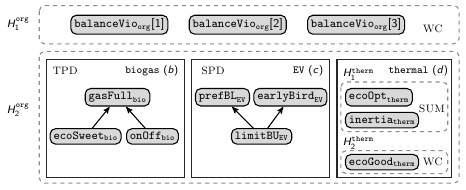
\includegraphics[width=.4\textwidth]{img/pvs.png} } };
% 
    \end{pgfonlayer}

\end{tikzpicture}

\end{figure}
\vspace*{-2.4ex}
\onslide<5->{\textbf{Ziel:} Integration von Individualpräferenzen.}
\end{frame}

\begin{frame}{Kombinationen~\cite{SchiendorferPvs2015}}
\fontsize{8pt}{7.2}\selectfont
\tikzset{
   main node/.style={rectangle,
                     rounded corners,
   					 fill=black!15,
   					 draw,
   					 minimum width=3.5em,
   					 text centered,
                     inner sep=2.5pt,	 
   					 font=\sffamily
   					},
   treestyle/.style={rectangle,fill=black!15,draw,font=\sffamily},
   constraint/.style={circle,fill=black!15,draw,font=\sffamily\small},
   constraint_satisfied/.style = {constraint, fill=white},
   constraint_violated/.style = {constraint, fill=black!25},
}

\begin{figure}[t]
\centering
\begin{tikzpicture}[->,>=stealth',shorten >=1pt,auto,node distance=1.45cm,inner sep=1.5pt,outer sep = 0.0pt, thick] 
%\tikzstyle{every node}=[font=\tiny]
\begin{scope}[xshift=-6.0cm,yshift=-4.0cm]
\node[main node, style={font=\sffamily\footnotesize}] at (0.1,1.5) {\minMaxViolation[1]};
\node[main node, style={font=\sffamily\footnotesize}] at (3.2,1.5) {\minMaxViolation[2]};
\node[main node, style={font=\sffamily\footnotesize}] at (6.3,1.5) {\minMaxViolation[3]};

\draw [rounded corners,dashed,black!45] (-2,2) rectangle (9.0,1);
\node[text width=3cm, anchor=west, right] at (-2.9, 1.5) { \hLevelOrg{1} };
\draw [rounded corners,dashed,black!45] (-2,0.8) rectangle (9.0,-2.65);
\node[text width=4cm, anchor=west, right] at (-2.9, -0.75) { \hLevelOrg{2} };

% bio
\draw [black!85,fill=forestgreen!35] (-1.8,0.6) rectangle (1.8,-2.5);
\node[main node, style={font=\sffamily\footnotesize}] (5) at (0.05,-0.4) {\gasFull};
\node[main node, style={font=\sffamily\footnotesize}] (6) [below left of=5,xshift=5.4] {\ecoSweet};
\node[main node, style={font=\sffamily\footnotesize}] (7) [below right of=5,xshift=-3.1] {\onOff};
%\node[main node, style={font=\sffamily\footnotesize},double] (hardConstraint) [below left of=7,xshift=-3.1,yshift=7] {$\mathsf{maxProd}$};
\node[text width=4cm, anchor=west, left] at (2.3, 0.3) { \textbf{ConstraintRel.:}  $\mathtt{\biogas}$ $(b)$ };
%\node[text width=2cm, anchor=west, left] at (0.4, 0.3) { CR \textsc{TPD} };

% EV
\draw [black!85,fill=black!35] (2.0,0.6) rectangle (5.6,-2.5);
\node[main node, style={font=\sffamily\footnotesize}] (3) at (2.80,-0.4) {\prefBatteryLevel};
\node[main node, style={font=\sffamily\footnotesize}] (4) at (4.58,-0.4)  {\earlyBird};
\node[main node, style={font=\sffamily\footnotesize}] (8) [below right of=3] {\limitBatteryUsage};
\node[text width=3cm, anchor=west, left] at (5.2, 0.3) { \textbf{ConstraintRel.:}  $\mathtt{\ev}$ $(c)$ };
%\node[text width=2cm, anchor=west, left] at (4.3, 0.3) { CR };
%\node[text width=1cm, anchor=east, left] at (5.3, -2.3) { \textsc{SPD} };

% thermal
\draw [black!85,fill=thermicred!25] (5.8,0.6) rectangle (8.8,-2.5);
\draw [rounded corners,dashed,black!45] (5.9,0) rectangle (8.7,-1.3);
\node[text width=4cm, anchor=west, right] at (5.9, 0.2) { \hLevelThermal{1} };
\draw [rounded corners,dashed,black!45] (5.9,-1.8) rectangle (8.7,-2.4);
\node[text width=4cm, anchor=west, right] at (5.9, -1.6) { \hLevelThermal{2} };
\node[main node, style={font=\ttfamily\footnotesize}] (10) at (6.9,-0.4) {\ecoOpt};
\node[main node, node distance=0.85cm, style={font=\sffamily\footnotesize}] (11) at (6.98,-1.0) {\inertia};
\node[main node, node distance=0.85cm, style={font=\sffamily\footnotesize}] (12) at (6.98,-2.1) {\ecoGood};
\node[text width=4cm, anchor=west, right] at (7.1, 0.3) { $\mathtt{\thermal}$ $(d)$ };

\node[text width=2cm, anchor=west, left] at (10, -0.7) { \textbf{CFN:} \\ $\mathtt{h1}$ };

\node[text width=2cm, anchor=west, left] at (10.1, -2.1) { \textbf{CFN:} \\ $\mathtt{h2}$ };

\node[text width=2cm, anchor=west, left] at (10.1, 1.4) { \textbf{CFN:} \\ $\mathtt{orga}$ };

\path[every node/.style={font=\sffamily\tiny}]
  (8) edge node [right] {} (3)
  (8) edge node [right] {} (4)
  (6) edge node [right] {} (5)
  (7) edge node [right] {} (5)
;
\end{scope}

% \begin{scope}[xshift=-0.2cm,yshift=-0.9cm]
% \node[text width=9cm,left] at (0.0, 0.0) {%
% \begin{itemize}[itemsep=2pt]
%   \item something interesting
% \end{itemize}
% };
% \end{scope}

\end{tikzpicture}
%\caption{Case study depicting individual and organizational preference specifications in context.}
\label{fig:preferencesCaseStudy}
\end{figure}
  



%%% Local Variables:
%%% mode: LaTeX
%%% mode: TeX-PDF
%%% mode: TeX-source-correlate
%%% TeX-master: "../quality-quantity-soft-constraints.tex"
%%% End:


\onslide<2->{
Die Bewertungsstruktur dieses Problems:
\vspace*{2ex}

\qquad $
  P_{\mathtt{org}_1} \ltimes (P_{\prosumer{\biogas}} \times P_{\prosumer{\ev}} \times (P_{\prosumer{\thermal}}^1 \ltimes P_{\prosumer{\thermal}}^2))
$
}
%
%\begin{textblock*}{7.5cm}[1,1](\textwidth+3.8cm,\textheight-0.13cm)
%\begin{itemize}
%%\item[] \textsc{SPD} \ldots Single-Pred.-Dom.
%%\item[] \textsc{TPD} \ldots Single-Pred.-Dom.
%\item[] \textsc{SUM} \ldots Sum of Errors
%\item[] \textsc{WC} \ldots Worst-Case Error
%
%
%\end{itemize}
% \end{textblock*}
\end{frame}
